\documentclass[10pt,a4paper,twoside]{report}
\usepackage{a4wide}
\usepackage[utf8]{inputenc}
\usepackage{verbatim}
\usepackage{amsmath}
\usepackage{amsfonts}
\usepackage{amssymb}
\usepackage{graphicx}
\usepackage{colortbl}
\author{Cyril Charron}

\definecolor{LightBlue}{rgb}{0.56,0.79,1}
\definecolor{LightYellow}{rgb}{0.99,1,0.79}

\title{Cheat Sheet for ORACLE Solaris 11 Course}
\begin{document}
\maketitle
\chapter{Introduction}
\chapter{Installing Oracle Solaris 11}
\section{Planning}
Planning is required to make sure that the operating system is installed properly and is configured to support business needs.
Planning addresses and answers such questions as:
\begin{itemize}
\item How many users will you need to support?
\item What applications will you be running?
\item What type of network will you be using?
\item What are your data storage needs?
\item What are your hardware needs?
\end{itemize}
\section{Installing}
\begin{table}
\begin{tabular}{|p{0.15\textwidth}|p{0.4\textwidth}|p{0.4\textwidth}|}
\hline
\rowcolor{LightBlue}
\textbf{Feature} & \textbf{Live Media GUI} & \textbf{Text Installer}\\
\hline
\rowcolor{LightYellow}
Packages & Installs desktop-based packages & Installs server-based set of packages\\
\hline
\rowcolor{LightYellow}
Network Configuration & Defaults to automatic network configuration & Allows both automatic and manual configuration of the network \\
\hline
\rowcolor{LightYellow}
root user & The root user is always configured as a role & The root user might not be a role \\
\hline
\rowcolor{LightYellow}
Memory & Requires more memory than text installer & Requires less memory than Live Media GUI installer\\
\hline
\end{tabular}
\end{table}
\section{Using an Interactive Installer}
Installing the operating system consists of four tasks:
\begin{enumerate}
\item Preparing for the installation
\item Preforming the installation
\item Verifying the installation
\item Rebooting the system
\end{enumerate}
\subsection{Preparing for the installation}
\begin{itemize}
\item Identify system requirements (disk space and memory)
\item Review additional installation considerations (whole-disk or partition)
\item Verify required device drivers
\end{itemize}
\textbf{Note}:\\
\begin{itemize}
\item the first user configured is given the \verb+root+ role.
\item after the reboot, you can find the installation log at \verb+/var/sadm/system/logs/install_log+ for the GUI install or \verb+/var/log/install/install_log+ for the text install.
\end{itemize}
\subsection{Baseline System Information Commands: Summary}
\begin{table}
\begin{tabular}{|p{0.65\textwidth}|p{0.3\textwidth}|}
\hline
\rowcolor{LightBlue}
\textbf{System Information} & \textbf{Command}\\
\hline
\rowcolor{LightYellow}
Host name & \verb+hostname+\\
\hline
\rowcolor{LightYellow}
Basic information: Operating system name, release, version, host name, hardware architecture and processor type & \verb+uname -a+\\
\hline
\rowcolor{LightYellow}
Operating system release information & \verb+cat /etc/release+\\
\hline
\rowcolor{LightYellow}
Disk configuration & \verb+format+\\
\hline
\rowcolor{LightYellow}
Installed memory & \verb+prtconf | grep Memory+\\
\hline
\rowcolor{LightYellow}
Information about network services & \verb+svcs network/physical+\\
\hline
\rowcolor{LightYellow}
Network interface information & \verb+ipadm show-addr+\\
\hline
\end{tabular}
\end{table}

\chapter{Updating and Managing Software Packages}
\section{Managing Software Packages by Using the Command-Line Interface and Package Manager}
List of know-how tasks:
\begin{itemize}
\item Searching for a package
\item Performing a test run on the package installation
\item Installing a package
\item Verifying the package installation
\item Displaying information about the package and its contents
\item Uninstalling a package
\end{itemize}

\begin{table}
\begin{tabular}{|p{0.65\textwidth}|p{0.3\textwidth}|}
\hline
\rowcolor{LightBlue}
\textbf{Package Management Task} & \textbf{IPS Command}\\
\hline
\rowcolor{LightYellow}
Display package state and version information & \verb+pkg list+\\
\hline
\rowcolor{LightYellow}
Display package information & \verb+pkg info+\\
\hline
\rowcolor{LightYellow}
Display content of a package & \verb+pkg conten+\\
\hline
\rowcolor{LightYellow}
Install package updates & \verb+pkg update+\\
\hline
\rowcolor{LightYellow}
Install package & \verb+pkg install+\\
\hline
\rowcolor{LightYellow}
Verify package installation & \verb+pkg verify+\\
\hline
\rowcolor{LightYellow}
Search for a package & \verb+pkg list+\\
\hline
\rowcolor{LightYellow}
Unistall a package & \verb+pkg list+\\
\hline
\end{tabular}
\caption{Package Management Commands: Summary}
\end{table}

\section{Boot Environment}
\begin{table}
\begin{tabular}{|p{0.55\textwidth}|p{0.4\textwidth}|}
\hline
\rowcolor{LightBlue}%{0.5,0.6,0.9}%{143,202,255}
\textbf{Boot Environment Task} & \textbf{Command}\\
\hline
\rowcolor{LightYellow}
List the boot environments on a system & \verb+beadm list+\\
\hline
\rowcolor{LightYellow}
Create a new boot environment & \verb+beadm create beName+\\
\hline
\rowcolor{LightYellow}
Rename a boot environment & \verb+beadm rename beName newBeName+\\
\hline
\rowcolor{LightYellow}
Destroy an inactive boot environment & \verb+beadm destroy beName+\\
\hline
\rowcolor{LightYellow}
Activate an inactive boot environment & {\verb+beadm activate beName+} {\verb+init 6+} \\
\hline
\end{tabular}
\end{table}

\chapter{Administering Services}
\section{Administering SMF Services}
\begin{table}[htbp]
\begin{tabular}{|p{0.4\textwidth}|p{0.55\textwidth}|}
\hline
\rowcolor{LightBlue}
 \textbf{SMF task}& \textbf{SMF Command} \\
\hline
\rowcolor{LightYellow}
List services currently running on the system & \verb+svcs+\\
\hline
\rowcolor{LightYellow}
List all the services defined on the system & \verb+svcs -a+\\
\hline
\rowcolor{LightYellow}
Display service dependents & \verb+svcs -D FMRI+\\
\hline
\rowcolor{LightYellow}
Display service dependencies & \verb+svcs -d FMRI+\\
\hline
\rowcolor{LightYellow}
Display the status of a service & \verb+svcs -l svc:/network/ssh:default+\\
\hline
\rowcolor{LightYellow}
Enable the SMF notification service & \verb+svcadm enable smtp-notify+\\
\hline
\rowcolor{LightYellow}
Disable a service & \verb+svcadm disable svc:/network/ssh:default+\\
\hline
\rowcolor{LightYellow}
Refresh a service & \verb+svcadm refresh svc:/network/ssh:default+\\
\hline
\rowcolor{LightYellow}
Restart a service & \verb+svcadm restart svc:/network/ssh:default+\\
\hline
\rowcolor{LightYellow}
Confirm the service is up and running & \verb+ps -ef | grep smtp-notify+\\
\hline
\rowcolor{LightYellow}
Configure the service state transition notification for all services monitored by SMF & \verb+svccfg -s svc:/system/svc/global:default+ \verb+setnotify -g service_transition_state+ \verb+mailto:root@localhost+\\
\hline
\rowcolor{LightYellow}
Configure notification for a single service & \verb+svccfg -s svc:/network/http:apache22+ \verb+ setnotify from-online mailto:root@localhost+\\
\hline
\rowcolor{LightYellow}
View configured notification & \verb+svccfg -s svc:/system/svc/global:default+ \verb+listnotify+\\
\hline
\rowcolor{LightYellow}
Stop all notifications & \verb+svccfg -s svc:/system/svc/global:default+ \verb+delnotify -g all+\\
\hline
\end{tabular}
\caption{Service Commands}
\end{table}

\textbf{Note:}
\begin{quote}
If the service is \verb+online+, the service dependencies are satisfied. If the service is not \verb+online+, use \verb+svcadm enable -r FMRI+ to recursively enable all dependencies.
\end{quote}

\textbf{Note:}
\begin{quote}
By default, the service \verb+svc:/system/boot-config:default+ is enabled with the property \verb+config/fastreboot_default+ set to \verb+true+. Running \verb+init 6+ will skip some firmware initialization steps and will skip the GRUB menu during reboot. The \verb+-p+ option appended to the \verb+reboot+ command disable the Fast Reboot feature.
\end{quote}

\begin{table}[htbp]
\begin{tabular}{|p{0.20\textwidth}|p{0.75\textwidth}|}
\hline
\rowcolor{LightBlue}
 \textbf{SMF task}& \textbf{SMF Command} \\
\hline
\rowcolor{LightYellow}
\verb+online+ & Enabled and successfully started.\\
\hline
\rowcolor{LightYellow}
\verb+offline+ & Enabled but not yet running or available to run.\\
\hline
\rowcolor{LightYellow}
\verb+disabled+ & Not enabled and not running.\\
\hline
\rowcolor{LightYellow}
\verb+legacy_run+ & Running. The legacy run is not managed by SMF, but the service can be observed.This state is used by legacy services only.\\
\hline
\rowcolor{LightYellow}
\verb+uninitialized+ & Starting up. This state is the initial state for all services before their configuration has been read.\\
\hline
\rowcolor{LightYellow}
\verb+maintenance+ & Error encountered that require administrative intervention.\\
\hline
\rowcolor{LightYellow}
\verb+degraded+ & Enabled but running at a limited capacity.\\
\hline
\end{tabular}
\caption{Service States}
\end{table}

\begin{table}[htbp]
\begin{tabular}{|p{0.47\textwidth}|p{0.48\textwidth}|}
\hline
\rowcolor{LightBlue}
\multicolumn{2}{|c|}{\textbf{Monitored Transition States}}\\
\hline
\rowcolor{LightYellow}
to-uninitialized & to-disabled\\
\hline
\rowcolor{LightYellow}
from-uninitialized & from-disabled\\
\hline
\rowcolor{LightYellow}
to-maintenance & to-online\\
\hline
\rowcolor{LightYellow}
from-maintenance & from-online\\
\hline
\rowcolor{LightYellow}
to-offline & to-degraded\\
\hline
\rowcolor{LightYellow}
from-offline & from-degraded\\
\hline
\end{tabular}
\caption{Service Transition States}
\end{table}
\section{Boot a System}
\subsection{Run Levels}

\begin{table}[htbp]
\begin{tabular}{|p{0.12\textwidth}|p{0.23\textwidth}|p{0.6\textwidth}|}
\hline
\rowcolor{LightBlue}
\textbf{Run Level} & \textbf{Resulting State} & \textbf{Description}\\
\hline
\rowcolor{LightYellow}
\verb+0+ & Exit the OS & The operating system is shut down, and it is safe to turn off power to the system.\\
\hline
\rowcolor{LightYellow}
\verb+s+ or \verb+S+ & Single-user state & A single user can log in. Some file systems are mounted and accessible.\\
\hline
\rowcolor{LightYellow}
\verb+2+ & Multiuser state & Multiple users can access the system and all file systems.\\
\hline
\rowcolor{LightYellow}
\verb+3+ & Multiuser level with server & All system resources are available, and multiple users can log in. This is the default run level.\\
\hline
\rowcolor{LightYellow}
\verb+5+ & Machine powers down & The system shuts down and then powers off the machine.\\
\hline
\rowcolor{LightYellow}
\verb+6+ & Boot to multiuser level with server & The system shuts down to system level \verb+0+ and then reboots to level \verb+3+.\\
\hline
\end{tabular}
\caption{Run Levels}
\end{table}

\begin{figure}
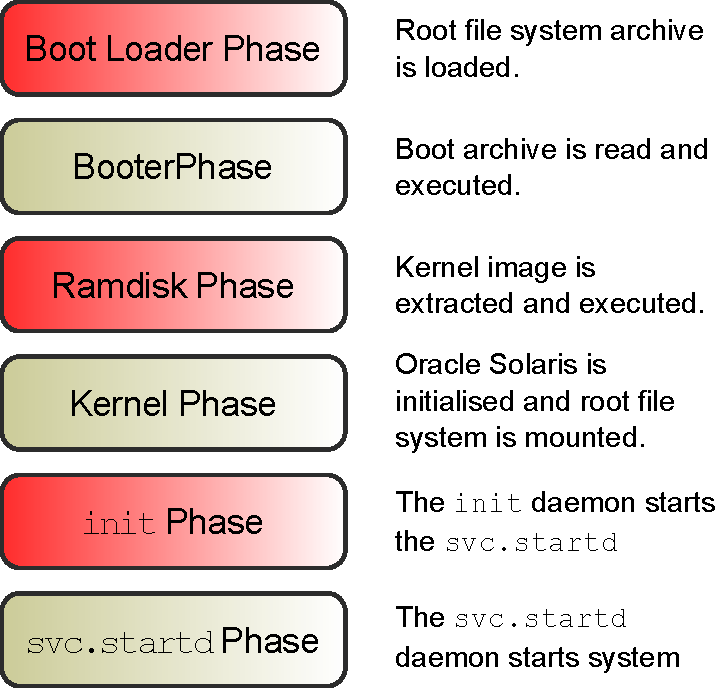
\includegraphics[height=0.4\textheight]{Solaris_BootSequence.pdf}
\caption{Boot process} 
\end{figure}
\subsection{Booting an x86 System to Run Level S (Single-User Milestone)}
\begin{enumerate}
\item Reboot the system by using the reboot -p command.
\item When the GRUB menu appears, enter e to edit the GRUB menu.
\item Use the arrow keys to choose the \verb+kernel $+ line.
\item Enter e again to edit the boot entry.
\item To boot the system in single-user mode, enter \verb+-s+ at the end of the boot entry line. Then press Return to go back to the previous screen.
\item To continue to boot the system in single-user mode, enter \verb+b+.
\item When prompted, enter the \verb+root+ password.
\item Verify that the system is at run level \verb+S+.
\end{enumerate}
\section{Shutdown a System}
\subsection{Shutting down a system}
\begin{itemize}
\item Shutting down a server:
\begin{itemize}
\item the \verb+shutdown+ command is used.
\item clean shutdown is performed.
\item superuser privileges are required.
\end{itemize}
\item Shutting down a stand-alone system:
\begin{itemize}
\item the \verb+init+ command is used.
\item clean shutdown is performed.
\item superuser privileges are required.
\end{itemize}
\end{itemize}
\begin{table}
\begin{tabular}{|p{0.15\textwidth}|p{0.8\textwidth}|}
\hline
\rowcolor{LightBlue}
 \textbf{Run Level}& \textbf{SMF Milestone FMRI} \\
\hline
\rowcolor{LightYellow}
\verb+S+ & \verb+milestone/single-user:default+\\
\hline
\rowcolor{LightYellow}
\verb+2+ & \verb+milestone/multi-user:default+\\
 \hline
\rowcolor{LightYellow}
\verb+3+ & \verb+milestone/multi-user/server:default+\\
 \hline
\end{tabular}
\end{table}


\chapter{Setting Up and Administering Data Storage}
\section{ZFS Pool}
\section{ZFS File Systems}
\section{ZFS Snapshots and Clones}
\chapter{Administering Oracle Solaris Zones}
\section{Determine the current zone configuration}
\section{Determine the current zone resource utilization}
\section{Administer an Oracle Solaris zone}
\chapter{Administering a Physical Network}
\chapter{Setting Up and Administering User Accounts}
\chapter{Controlling Access to Systems and Files}
\chapter{Managing System Processes and Scheduling System Tasks}
\chapter{Performing Basic System Monitoring and Troubleshooting}
\end{document}